\documentclass[a4paper]{article}
\usepackage{geometry}
\usepackage{graphicx}
\usepackage{natbib}
\usepackage{amsmath}
\usepackage{amssymb}
\usepackage{amsthm}
\usepackage{paralist}
\usepackage{epstopdf}
\usepackage{tabularx}
\usepackage{longtable}
\usepackage{multirow}
\usepackage{multicol}
\usepackage[hidelinks]{hyperref}
\usepackage{fancyvrb}
\usepackage{float}
\usepackage{paralist}
\usepackage[svgname]{xcolor}
\usepackage{enumerate}
\usepackage{array}
\usepackage{times}
\usepackage{url}
\usepackage{fancyhdr}
\usepackage{comment}
\usepackage{environ}
\usepackage{times}
\usepackage{textcomp}
\usepackage{caption}
\usepackage{bbm}
\usepackage{enumitem}
\usepackage{algorithm}
\usepackage{algpseudocode}
\usepackage{caption}
\usepackage{subcaption}


\urlstyle{rm}

\setlength\parindent{0pt} % Removes all indentation from paragraphs
\theoremstyle{definition}
\newtheorem{definition}{Definition}[]
\newtheorem{conjecture}{Conjecture}[]
\newtheorem{example}{Example}[]
\newtheorem{theorem}{Theorem}[]
\newtheorem{lemma}{Lemma}
\newtheorem{proposition}{Proposition}
\newtheorem{corollary}{Corollary}

\floatname{algorithm}{Procedure}
\renewcommand{\algorithmicrequire}{\textbf{Input:}}
\renewcommand{\algorithmicensure}{\textbf{Output:}}
\newcommand{\abs}[1]{\lvert#1\rvert}
\newcommand{\norm}[1]{\lVert#1\rVert}
\newcommand{\RR}{\mathbb{R}}
\newcommand{\CC}{\mathbb{C}}
\newcommand{\Nat}{\mathbb{N}}
\newcommand{\br}[1]{\{#1\}}
\DeclareMathOperator*{\argmin}{arg\,min}
\DeclareMathOperator*{\argmax}{arg\,max}
\renewcommand{\qedsymbol}{$\blacksquare$}

\definecolor{dkgreen}{rgb}{0,0.6,0}
\definecolor{gray}{rgb}{0.5,0.5,0.5}
\definecolor{mauve}{rgb}{0.58,0,0.82}

\newcommand{\Var}{\mathrm{Var}}
\newcommand{\Cov}{\mathrm{Cov}}

\newcommand{\vc}[1]{\boldsymbol{#1}}
\newcommand{\xv}{\vc{x}}
\newcommand{\Sigmav}{\vc{\Sigma}}
\newcommand{\alphav}{\vc{\alpha}}
\newcommand{\muv}{\vc{\mu}}

\newcommand{\red}[1]{\textcolor{red}{#1}}

\def\x{\mathbf x}
\def\y{\mathbf y}
\def\w{\mathbf w}
\def\v{\mathbf v}
\def\E{\mathbb E}
\def\V{\mathbb V}
\def\ind{\mathbbm 1}

% TO SHOW SOLUTIONS, include following (else comment out):
\newenvironment{soln}{
	\leavevmode\color{blue}\ignorespaces
}{}

\hypersetup{
	%    colorlinks,
	linkcolor={red!50!black},
	citecolor={blue!50!black},
	urlcolor={blue!80!black}
}

\geometry{
	top=1in,            % <-- you want to adjust this
	inner=1in,
	outer=1in,
	bottom=1in,
	headheight=3em,       % <-- and this
	headsep=2em,          % <-- and this
	footskip=3em,
}


\pagestyle{fancyplain}
\lhead{\fancyplain{}{Homework 6}}
\rhead{\fancyplain{}{CS 760 Machine Learning}}
\cfoot{\thepage}

\title{\textsc{Homework 6}} % Title

%%% NOTE:  Replace 'NAME HERE' etc., and delete any "\red{}" wrappers (so it won't show up as red)

\author{
	\red{$>>$NAME HERE$<<$} \\
	\red{$>>$ID HERE$<<$}\\
} 

\date{}

\begin{document}
	
	\maketitle 
	
        \textbf{Instructions:}
        Use this latex file as a template to develop your homework. We are changing our reproducibility policy on code submissions going forward. \textbf{Instead of uploading it on GitHub, please submit a separate zip file that contains your code. You will submit two files to Canvas, one is your pdf, and the other one is a zip file.} Late submissions may not be accepted. You can choose any programming language (i.e. python, R, or MATLAB). Please check Piazza for updates about the homework.
        \vspace{0.1in}
	
	\section{Implementation: GAN (30 pts)}
	In this part, you are expected to implement GAN with MNIST dataset. We have provided a base jupyter notebook (gan-base.ipynb) for you to start with, which provides a model setup and training configurations to train GAN with MNIST dataset.
	
	\begin{enumerate} [label=(\alph*)]
		\item Implement training loop and report learning curves and generated images in epoch 1, 50, 100. Note that drawing learning curves and visualization of images are already implemented in provided jupyter notebook. \hfill (15 pts)
		
		\begin{algorithm}
			\caption{Training GAN, modified from \cite{goodfellow2014generative}}\label{alg:GAN}
			\begin{algorithmic}
				\Require $m$: real data batch size, $n_{z}$: fake data batch size
				\Ensure Discriminator $D$, Generator $G$
				
				\For{number of training iterations}
				
				\State{$\#$ Training discriminator}
				\State{Sample minibatch of $n_{z}$ noise samples $\{z^{(1)}, z^{(2)}, \cdots, z^{(n_{z})}\}$ from noise prior $p_{g}(z)$}
				\State{Sample minibatch of $\{x^{(1)}, x^{(2)}, \cdots, x^{(m)}\}$}
				\State{Update the discriminator by ascending its stochastic  gradient:
					$$\nabla_{\theta_{d}} \big ( \cfrac{1}{m}  \sum_{i=1}^{m}  \log D(x^{(i)})  + \cfrac{1}{n_{z}} \sum_{i=1}^{n_{z}}  \log (1-D(G(z^{(i)})))\big )$$
				}
				
				\State{$\#$ Training generator}
				\State{Sample minibatch of $n_{z}$ noise samples $\{z^{(1)}, z^{(2)}, \cdots, z^{(n_{z})}\}$ from noise prior $p_{g}(z)$}
				\State{Update the generator  by ascending its stochastic  gradient:
					$$\nabla_{\theta_{g}}  \cfrac{1}{n_{z}} \sum_{i=1}^{n_{z}}  \log D(G(z^{(i)}))\big )$$
				}
				\EndFor
				
				\State{$\#$ The gradient-based updates can use any standard gradient-based learning rule. In the base code, we are using Adam optimizer \citep{kingma2014adam}}
			\end{algorithmic}
		\end{algorithm}
		
		Expected results are as follows.
		
		\begin{figure}[H]
			\centering
			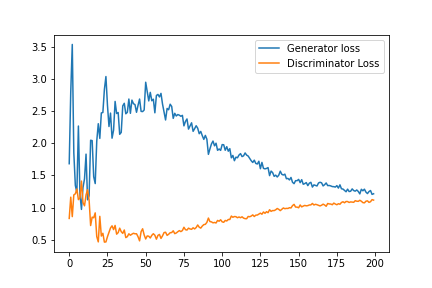
\includegraphics[width=0.7\textwidth]{gan_q1_loss.png}
			\caption{Learning curve}
			\label{fig:gan_q1_loss}
		\end{figure}
		
		\begin{figure}[H]
			\centering
			\begin{subfigure}[b]{0.3\textwidth}
				\centering
				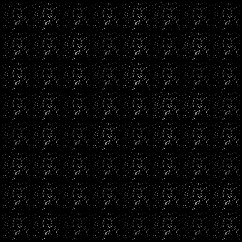
\includegraphics[width=\textwidth]{gan_q1_epoch1.png}
				\caption{epoch 1}
			\end{subfigure}
			\hfill
			\begin{subfigure}[b]{0.3\textwidth}
				\centering
				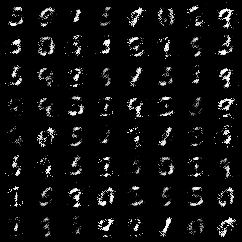
\includegraphics[width=\textwidth]{gan_q1_epoch50.png}
				\caption{epoch 50}
			\end{subfigure}
			\hfill
			\begin{subfigure}[b]{0.3\textwidth}
				\centering
				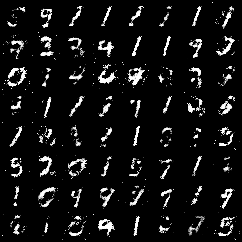
\includegraphics[width=\textwidth]{gan_q1_epoch100.png}
				\caption{epoch 100}
			\end{subfigure}
			\caption{Generated images by $G$}
			\label{fig:three graphs}
		\end{figure}
		
		
		\begin{soln}  Solution goes here. Attach your learning curve and images. \end{soln}
		
		
		
		\item Replace the generator update rule as the original one in the slide,\\
		``Update the generator by descending its stochastic gradient:
		
		$$\nabla_{\theta_{g}}  \cfrac{1}{n_{z}}  \sum_{i=1}^{n_{z}}\log (1-D(G(z^{(i)})))\big )$$
		"
		, and report learning curves and generated images in epoch 1, 50, 100. Compare the result with (a). Note that it may not work. If training does not work, explain why it doesn't work.
		\hfill (10 pts)
		
		\begin{soln}  Solution goes here. Attach your learning curve and images. \end{soln}
		
		\item Except the method that we used in (a), how can we improve training for GAN? Implement that and report your setup, learning curves, and generated images in epoch 1, 50, 100.
		\hfill (5 pts)
		
		\begin{soln}  Solution goes here. Attach your learning curve and images. \end{soln}
		
	\end{enumerate}

	\section{Review change of variables in probability density functions [25 pts]} In Flow based generative model, we have seen $p_{\theta}(x)=p(f_{\theta}(x))|\frac{\partial f_{\theta}(x)}{\partial x}|$. As a hands-on (fixed parameter) example, consider the following setting.\\
	Let $X$ and $Y$ be independent, standard normal random variables. Consider the transformation $U=X+Y$ and $V=X-Y$. In the notation used above, $U=g_{1}(X, Y)$ where $g_{1}(X, Y)$ where $g_{1}(x, y)=x+y$ and $V=g_{2}(X, Y)$ where $g_{2}(x,y)=x-y$. The joint pdf of $X$ and $Y$ is $f_{X, Y}=(2\pi)^{-1} exp(-x^{2}/2) exp(-y^{2}/2), -\infty < x < \infty, -\infty < y < \infty$. Then, we can determine $u, v$ values by $x, y$, i.e. 
	$
	\begin{bmatrix}
		u\\
		v
	\end{bmatrix}
	$
	$=\begin{bmatrix}
		1 & 1 \\ 
		1 & -1
	\end{bmatrix}
	$
	$
	\begin{bmatrix}
		x\\
		y
	\end{bmatrix}
	$
	.
	
	\begin{enumerate}[label=(\alph*)]
		\item Compute Jacobian matrix $$J=\begin{bmatrix}
			\cfrac{\partial x}{\partial u} & \cfrac{\partial x}{\partial v}\\
			\cfrac{\partial y}{\partial u} & \cfrac{\partial y}{\partial v}
		\end{bmatrix}
		$$
		\hfill (5 pts)
		
		\begin{soln}  Solution goes here. \end{soln}
		
		
		\item (Forward) Show that the joint pdf of U, V is
		$$f_{U, V}(u, v)=\big (\cfrac{1}{\sqrt{2\pi}\sqrt{2}}exp(-u^{2}/4)\big ) \big (\cfrac{1}{\sqrt{2\pi}\sqrt{2}}exp(-v^{2}/4)\big )$$
		\hfill (10 pts) \\
		(Hint: $f_{U, V}(u, v)=f_{X, Y}(?, ?)|det(J)|$) \\
		
		\begin{soln}  Solution goes here. \end{soln}
		
		\item (Inverse) Check whether the following equation holds or not.
		$$f_{X, Y}(x, y)=f_{U, V}(x+y, x-y)|det(J)^{-1}|$$
		
		\hfill (10 pts) 
		
		\begin{soln}  Solution goes here. \end{soln}
	\end{enumerate}

\section{Directed Graphical Model [20 points]}
Consider the directed graphical model (aka Bayesian network) in Figure~\ref{fig:bn}.
\begin{figure}[H]
    \centering
    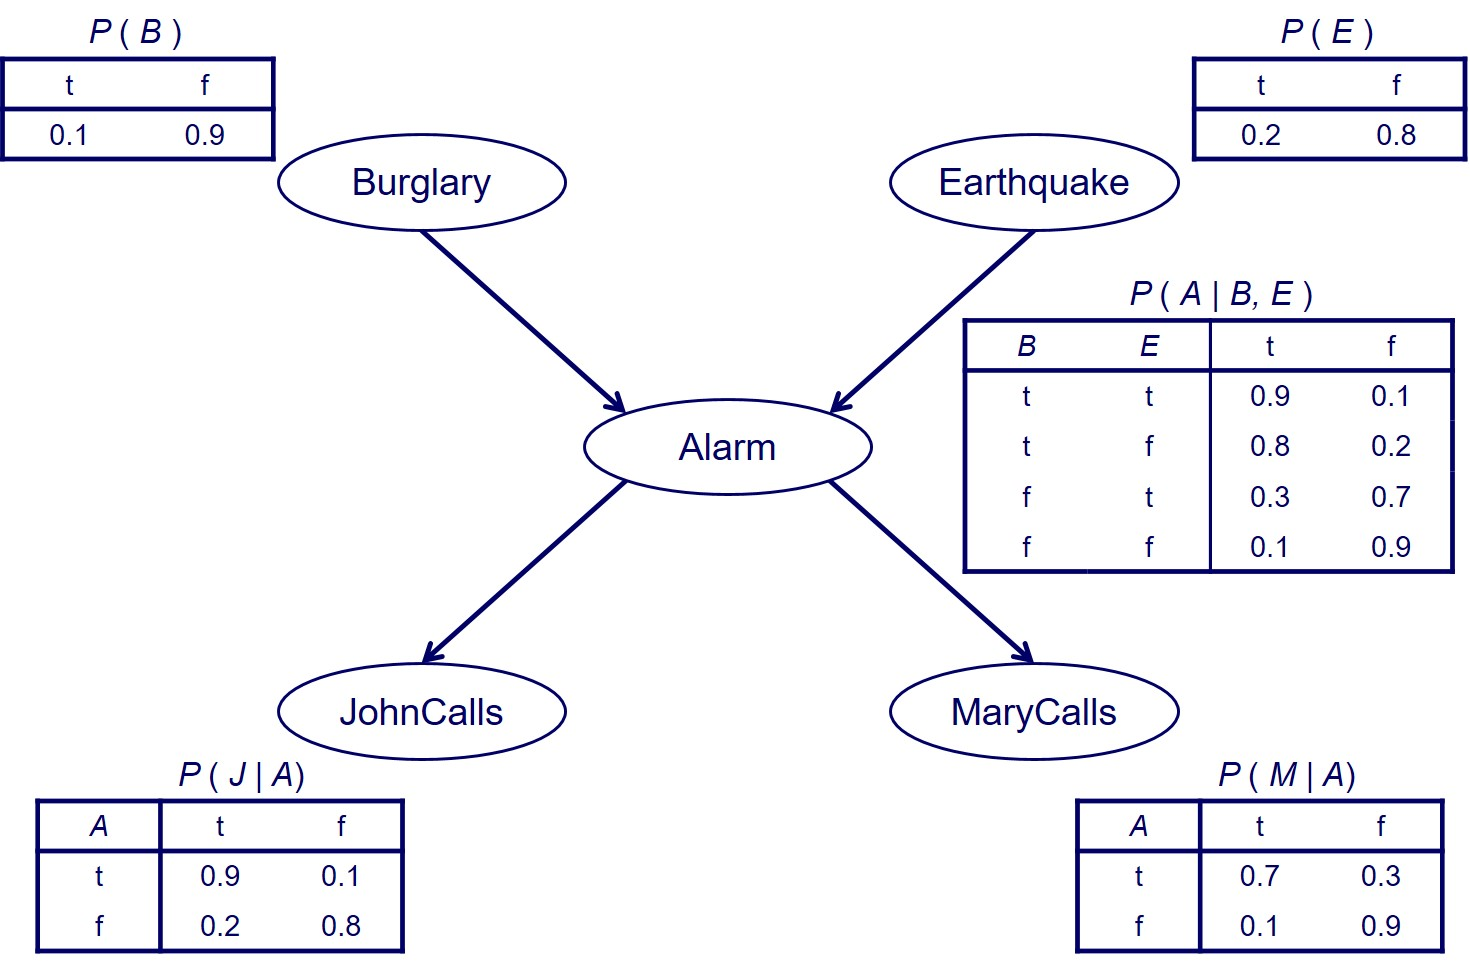
\includegraphics[width=0.8\textwidth]{BN.jpg}
    \caption{A Bayesian Network example.}
    \label{fig:bn}
\end{figure}
Compute $P(B=t \mid E=f,J=t,M=t)$ and $P(B=t \mid E=t,J=t,M=t)$. (10 points for each) These are the conditional probabilities of a burglar in your house (yikes!) when both of your neighbors John and Mary call you and say they hear an alarm in your house, but without or with an earthquake also going on in that area (what a busy day), respectively.

\begin{soln}  Solution goes here. \end{soln}


\section{Chow-Liu Algorithm [25 pts]}
Suppose we wish to construct a directed graphical model for 3 features $X$, $Y$, and $Z$ using the Chow-Liu algorithm. We are given data from 100 independent experiments where each feature is binary and takes value $T$ or $F$. Below is a table summarizing the observations of the experiment:

\begin{table}[H]
        \centering
                \begin{tabular}{cccc}
                           $X$ & $Y$ & $Z$ & Count \\
                                \hline
                                T & T & T & 36 \\
                                \hline
                                T & T & F & 4 \\
                                \hline
                                T & F & T & 2 \\
                                \hline
                                T & F & F & 8 \\
                                \hline
                                F & T & T & 9 \\
                                \hline
                                F & T & F & 1 \\
                                \hline
                                F & F & T & 8 \\
                                \hline
                                F & F & F & 32 \\
                                \hline
                \end{tabular}
\end{table}

\begin{enumerate}
	\item Compute the mutual information $I(X, Y)$ based on the frequencies observed in the data. (5 pts)
	\item Compute the mutual information $I(X, Z)$ based on the frequencies observed in the data. (5 pts)
	\item Compute the mutual information $I(Z, Y)$ based on the frequencies observed in the data. (5 pts)
	\item Which undirected edges will be selected by the Chow-Liu algorithm as the maximum spanning tree? (5 pts)
	\item Root your tree at node $X$, assign directions to the selected edges. (5 pts)
\end{enumerate}

	\bibliography{hw6}
	\bibliographystyle{apalike}
\end{document}
